%
% Documento: Desenvolvimento
%

\chapter{Desenvolvimento}

O desenvolvimento desse trabalho passou por três etapas principais, a configuração do servidor de teste, a implementação dos testes e a execução dos testes. Neste capítulo serão descritos os detalhes dessas três etapas e as dificuldades encontradas em cada uma delas.

\section{O servidor}
\label{oservidor}

Em poucas palavras, um servidor é um programa de computador que recebe requisições e envia respostas. Na \textit{Web}, o tipo mais comum de requisição e resposta são as requisições e respostas HTTP. Sendo assim, a função primaria de um servidor \textit{web} é aguardar por requisições HTTP e servir páginas \textit{web}.

Os servidores \textit{web} mais populares do mundo atualmente são o Apache\footnote{http://www.apache.org/} e o Nginx\footnote{http://nginx.org/}.

\subsection{Apache}
\label{apache}

O servidor \textit{web} Apache foi lançado em 1995 por um grupo de entusiastas que procuravam uma maneira segura, eficiente e escalável de servir páginas \textit{web} para todos.  De acordo com \citeonline{ApacheHTTPD}, o servidor Apache se tornou o mais popular do mundo em Abril de 1996 e nunca mais perdeu essa posição. Desde o início, o projeto se desenvolveu como uma iniciativa de código livre e assim se mantém até os dias atuais. As grandes vantagens do Apache são que ele pode ser executado em qualquer sistema operacional UNIX\footnote{Família de sistemas operacionais que é utilizado como base do Linux e do iOS. https://en.wikipedia.org/wiki/Unix} ou Windows NT\footnote{Família de sistemas operacionais produzidas pelas \textit{Microsoft}. https://en.wikipedia.org/wiki/Windows\_NT} e é simples de ser configurado.

\subsection{Nginx}
\label{nginx}

Assim como o Apache, o Nginx é um projeto de código livre de servidor HTTP. Começou a ser desenvolvido em 2002 e teve sua primeira versão pública lançada em 2004. A motivação para a criação do Nginx foi encontrar uma solução para o problema C10K\footnote{http://www.kegel.com/c10k.html}, que diz que um servidor \textit{web} deve suportar 10 mil conexões paralelas. Sendo assim, como explica \citeonline{Nginx}, o servidor foi construído com um arquitetura completamente assíncrona que beneficia de pequenos serviços de hospedagem à grandes sistemas de computação paralela.

\subsection{A escolha do servidor}
\label{aescolhadoservidor}

Para executar os testes propostos foi necessário utilizar um servidor que suportasse tanto requisições HTTP/1.1 quanto HTTP/2. Como o HTTP/2 ainda é recente, encontrar um servidor com tal característica se mostrou um grande desafio.

Existem várias implementações do protocolo no mercado, cada uma com características diferentes e em estados diferentes de maturidade\footnote{Para obter mais informações sobre as diferentes implementações do HTTP/2 acesse o link a seguir. https://github.com/http2/http2-spec/wiki/Implementations}. Mas o grande problema é que a grande maioria dessas implementações são privadas e especificas para as empresas que as desenvolveram. Para o Apache e o Nginx ainda não foram lançadas versões oficiais do protocolo.

Apesar de não existir uma versão oficial do HTTP/2 para o Apache, existe um projeto de código aberto chamado \textit{mod\_h2}, desenvolvido por \citeonline{ModH2}, que se tornará a versão oficial do protocolo quando atingir um nível de maturidade e estabilidade considerado aceitável pela Apache Foundation. Já para o Nginx, não existe ainda uma extensão oficial nem um projeto de grande porte que implemente o novo protocolo dentro do servidor. Sendo assim o Apache seria a melhor escolha de servidor de teste.

As instruções para a instalação do mod\_h2 podem ser encontradas no site oficial do módulo e incluem:
\begin{enumerate}
	\item Baixar os arquivos do projeto
	\item Gerar arquivos de configuração e construção do módulo
	\item Compilar o módulo
	\item Mudar configurações do Apache para utilizar o novo módulo
	\item Ativar suporte ao novo protocolo
\end{enumerate}

Apesar da simplicidade, após várias tentativas, não foi concluir a configuração do módulo. Os arquivos foram compilados e foi gerado o arquivo executável necessário para a utilização do mod\_h2. Sendo assim, o próximo passo seria configurar o servidor para utilizar o novo protocolo como preferencial nas requisições e respostas HTTP. Mas, apesar de seguir todas as instruções descritas no site do mod\_h2, não foi possível fazer com que o Apache executasse o HTTP/2. O processo final utilizado está descrito no \autoref{apend:tentativadeconfiguracaomodh2}.

Como a configuração do servidor Apache falhou e o Nginx ainda não possuí suporte para o HTTP/2, foi necessário encontrar uma solução alternativa para executar o protocolo.

\subsubsection{O nghttp2}
\label{onghttp2}

O \textit{nghttp}, desenvolvido por \citeonline{nghttp}, é uma implementação em linguagem C do HTTP/2 e do protocolo de compressão HPACK. Essa implementação possui um cliente, um servidor, um \textit{proxy} e uma ferramente de teste para o servidor. O próprio mod\_h2, escolhido para ser o módulo oficial do Apache, usa o \textit{nghttp2} como base de sua implementação. Apesar do nome sugerir que existe alguma ligação entre o Nginx e o \textit{nghttp2}, não foi possível encontrar nada que relacione os dois servidores.

Apesar de os passos para a instalação do \textit{nghttp2} estarem documentados no site do projeto, algumas etapas importantes sobre instalação de dependências necessárias para fazer a aplicação funcionar corretamente não estão bem explicadas. Sendo assim, foram encontradas dificuldades no processo de instalação. Mas após superar essas dificuldades a aplicação foi configurada e foi possível confirmar seu funcionamento com a ajuda de um navegador que estava aceitando requisições e respostas HTTP/2. O processo de instalação está descrito no \autoref{apend:configurandonghttp2}.

\subsubsection{Escolha final}
\label{escolhafinal}

Apesar dos esforços para encontrar um servidor que suportasse às várias versões do protocolo HTTP, tal feito não foi possível. Sendo assim, ficou decido que seriam utilizados dois servidores diferentes para a realização dos testes, um para o HTTP/1.1 e outro para o HTTP/2.

Como o \textit{nghttp2} foi o único servidor com suporte ao HTTP/2 que a instalação foi feita com sucesso, ele foi escolhido como o servidor de teste para o novo protocolo. E por apresentar performance melhor do que o Apache, o Nginx foi escolhido como o servidor de teste para o HTTP/1.1.


\section{Descrição dos testes}
\label{descricaodostestes}

Os testes foram realizados em navegadores \textit{web}, o que torna o processo independente do sistema operacional. Mas o servidor foi configurado em uma máquina utilizando o sistema Ubuntu 14.04LTS, sendo assim, vale ressaltar, que os comandos descritos não vão necessariamente funcionar em sistemas operacionais diferentes do utilizado neste trabalho.

\subsection{Considerações inicias}
\label{consideracoesiniciais}

O nghttp2 permite a escolha do uso de HTTP/2 de duas maneiras:
\begin{enumerate}
	\item Utilização do \textit{nghttpx} para a criação de um \textit{proxy} para servidor HTTP/1.1
	\item Utilização do servidor \textit{nghttpd}
\end{enumerate}

Utilizar a primeira opção significa que o navegador vai mandar uma requisição HTTP/2 para a porta que o \textit{proxy} está escutando. Essa requisição vai então ser traduzida para pelo \textit{proxy}, que vai transforma-lá em uma requisição HTTP/1.1 e vai redireciona-lá para o servidor HTTP/1.1 que está escutando outra porta. O servidor HTTP/1.1 vai fazer todas as tarefas necessárias e vai retornar uma resposta HTTP/1.1 para o \textit{proxy}, que vai traduzi-la de volta para o HTTP/2 e retorna-la para o navegador. Esse processo está ilustrado na ADICIONAR FIGURA.

Apesar de parecer muito custoso, a implementação desse \textit{proxy} já garante ao usuário uma melhora de desempenho de seu servidor, isso porque a comunicação HTTP/2 é mais rápida e melhora o paralelismos das conexões. Além disso, o \textit{proxy} ainda possibilita o uso de funcionalidades especificas do HTTP/2, como o \textit{Server Push}.

A segunda opção utiliza o servidor embutido dentro do nghttp para fazer todo o trabalho. Dessa forma o navegador se comunica com esse servidor que faz todo o processamento necessário e retorna a resposta para o navegador. Tudo isso utilizando o protocolo HTTP/2. A desvantagem desse método é que o \textit{nghttpd} não possui um arquivo de configuração, o que é uma característica típica de servidores como o Apache e o Nginx, e por isso ele acaba sendo limitado em alguns casos. Por exemplo, ainda não é possível utilizar o \textit{Server Push} com o \textit{nghttpd}, pois para configurar essa funcionalidade é necessário um arquivo de configuração.

Como os servidores de teste para cada protocolo já são diferentes, houve um grande esforço para deixar as outras configurações do ambiente as mais similares possíveis, tentando evitar diferenças de desempenho. Sendo assim a escolha pela configuração utilizando o \textit{nghttpx} foi descartada. O redirecionamento via \textit{proxy} acrescentaria mais uma etapa no processo de comunicação cliente-servidor, e mesmo que se um outro \textit{proxy} fosse configurado para o servidor HTTP/1.1, ainda assim existe a etapa de tradução que não teria como ser simulada. Com isso, a configuração escolhida foi o uso do \textit{nghttpd}.

Como dito anteriormente, apesar de o HTTP/2 ter sido pensado inicialmente para funcionar apenas sob o protocolo TLS para melhorar a segurança da \textit{Web}, essa proposta não foi aprovada e o protocolo pode ser executado tanto com certificados de segurança como sem. Sendo assim, a intenção inicial era executar os testes nos dois ambientes, HTTP e HTTPS, contudo o \textit{nghttpd} não funcionou corretamente quando o certificado de segurança foi retirado e por isso os testes foram executados apenas com o protocolo HTTPS. Esse tipo de falha no servidor, embora seja um problema para aplicações que querem utilizar do novo protocolo, são esperadas, pois a tecnologia ainda é muito nova e não houve tempo ábil para corrigir todos os erros.

\subsection{Utilizando o \textit{nghttpd}}
\label{utilizandoonghttpd}

Para utilizar o \textit{nghttpd} é necessário uma porta possa ser escutada pelo novo servidor, um arquivo de certificado digital e uma chave para tal certificado. Então, tendo o \textit{nghttp2} instalado basta executar o seguinte comando:

\textbf{sudo nghttpd 83 /etc/apache2/ssl/dreamtech.key /etc/apache2/ssl/dreamtech.crt -d/var/www/html/tcc -v}

\begin{itemize}
	\item 83 define qual porta será escutada pelo servidor
	\item /etc/apache2/ssl/dreamtech.key é o caminho para o arquivo de chave do certificado digital
	\item /etc/apache2/ssl/dreamtech.crt é o caminho para o certificado digital
	\item -d define que uma pasta diferente da atual será servido pelo servidor
	\item /var/www/html/tcc é o caminho da pasta que será servida
	\item -v define que o servidor deverá exibir (verbalizar) as operações que está executando
\end{itemize}

Com isso o servidor para o protocolo HTTP/2 já está funcionando, apontando para a pasta /var/www/html/tcc e já pode ser acessado pela porta 83.

\subsection{Técnicas Escolhidas}
\label{tecnicasescolhidas}

Após análise das técnicas propostas por Steven Souders em seus livros, foi concluído que cinco técnicas podem sofrer alterações com a implantação do novo protocolo. São essas:

\begin{enumerate}
	\item Faça menos requisições HTTP
	\item Reduza o número de pesquisas DNS
	\item Evite redirecionamentos
	\item Lidando com \textit{scripts} assíncronos
	\item Quebrando domínios dominantes
\end{enumerate}

Das cinco técnicas listadas acima apenas três puderão ser testadas. Isso porque para testar a técnica 3 (três) é necessário um arquivo de configurações, o que ainda não é suportado pelo \textit{nghttpd} e a funcionalidade que melhorará o desempenho da técnica 4 (quatro) ainda não foi implementada no \textit{nghttp2}.

Sendo assim apenas três técnicas propostas por Steven Souder foram testadas. Mas, para complementar a análise da melhora de desempenho causada pelo HTTP/2, um quarto teste foi feito utilizando um \textit{template} pronto e simplesmente o executando no HTTP/1.1 e depois no HTTP/2.

Para cada teste foram criados projetos HTML separados, dessa forma o comportamento de uma técnica não interfere na outra. Além disso foram escolhidos arquivos CSS e \textit{javascript} de maneira aleatória para a realização dos testes. Esses arquivos são de bibliotecas famosas e não foram alterados, apenas concatenados na realização de testes que necessitavam minificação. As bibliotecas escolhidas foram:

\begin{itemize}
	\item Animate CSS: \textit{https://daneden.github.io/animate.css/}
	\item Bootstrap: \textit{http://getbootstrap.com/}
	\item JQuery: \textit{https://jquery.com/}
	\item Font Awesome: \textit{https://fortawesome.github.io/Font-Awesome/}
	\item Full Calendar: \textit{http://fullcalendar.io/}
	\item Normalize: \textit{https://necolas.github.io/normalize.css/}
	\item Skeleton: \textit{http://getskeleton.com/}
	\item Angular JS: \textit{https://angularjs.org/}
	\item Backbone JS: \textit{http://backbonejs.org/}
	\item D3: \textit{http://d3js.org/}
	\item Ember JS: \textit{http://emberjs.com/}
	\item High Charts: \textit{http://www.highcharts.com/}
	\item Moment JS: \textit{http://momentjs.com/}
	\item Require JS: \textit{http://requirejs.org/}
\end{itemize}

Abaixo encontram-se a explicações de cada teste e os códigos fontes podem ser encontrados anexados ao final deste trabalho.

\subsubsection{Faça menos requisições HTTP}
\label{facamenosrequisicoeshttp}

Para a realização desse teste vários arquivos CSS e \textit{javascript} foram inseridos na página. Primeiramente os arquivos são inseridos separadamente e depois são concatenados e inseridos de uma só vez. A soma dos tamanhos dos arquivos separados é 285kB maior do que a soma dos arquivos concatenados, isso ocorre por causa da remoção de espaços em branco.

Com o intuito de estressar a conexão simulando melhor o número de requisições de um site real, foram inseridas na página 28 imagens de diferentes tamanhos e formatos. Essa imagens são aleatórias e nunca são alteradas.

O código para o teste com arquivos separados pode ser encontrado no \autoref{apend:codigo_facamenosrequisicoeshttp_sep} e o código para o teste com os arquivos concatenados no \autoref{apend:codigo_facamenosrequisicoeshttp_concat}.

\subsubsection{Reduza o número de pesquisas DNS}
\label{reduzaonumerodepesquisasdns}

Nesse teste os mesmos arquivos CSS e \textit{javascript} do teste \ref{facamenosrequisicoeshttp} foram utilizados, mas dessa vez, ao invés de serem hospedados juntamente com o arquivo HTML, eles foram inseridos via CDN. Sendo assim a diferença está no numero de CDNs utilizadas. Enquanto no código do \autoref{apend:codigo_reduzaonumerodepesquisasdns_mult} são utilizadas 4 CNDs diferentes, no código do \autoref{apend:codigo_reduzaonumerodepesquisasdns_unic} apenas uma é utilizada. Com isso, no primeiro teste são feitas quatro consultas de DNS e no segundo apenas uma.

\subsubsection{Quebrando domínios dominantes}
\label{quebrandodominiosdominantes}

Enquanto que no teste \autoref{reduzaonumerodepesquisasdns} o número de pesquisas de DNS vai um extremo ao outro, passa de 4 para 1, nesse teste as medições são repetidas para 2 e 3 DNS diferentes na página, com o intuito de se encontrar o número ideal de consultas de DNS que diminui o tempo de pesquisas e aumenta o paralelismo das requisições. O código para esse teste encontra-se no \autoref{apend:quebrandodominiodominantes}.

\subsection{Realização dos testes}
\label{realizacaodostestes}

Para iniciar os testes foi necessário garantir que os navegadores escolhidos estavam com a opção de realizar requisições HTTP/2 habilitada. Enquanto que no Google Chrome está opção já vem habilitada por padrão e não existe mais jeito de desabilita-la, no Mozilla Firefox foi necessário seguir o procedimento descrito à seguir para garantir que o navegador fizesse as requisições com o novo protocolo.

\begin{enumerate}
	\item Digite \textit{about:config} na barra de navegação
	\item Confirme que deseja alterar as configurações do seu navegador
	\item Na barra de pesquisa, procure por \textit{network.http.spdy.enabled.http2draft}
	\item Clique duas vezes na preferência e confirma que seu resultado foi alterado para verdadeiro
	\item Na barra de pesquisa, procure por \textit{security.ssl.enable\_alpn}
	\item Clique duas vezes na preferência e confirma que seu resultado foi alterado para verdadeiro	
\end{enumerate}

Em seguida, para garantir que os navegadores estavam fazendo requisições HTTP/2, bastou iniciar o servidor \textit{nghttpd} e utilizar as ferramentas de desenvolvedor de cada navegador.

\begin{figure}[!htb]
    \centering
    \caption{Ferramentas do desenvolvedor do Google Chrome mostrando protocolo usado na requisição.}
    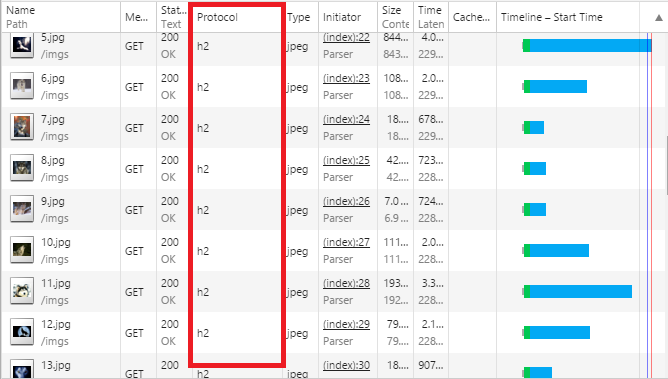
\includegraphics[width=0.7\textwidth]{./04-figuras/desenvolvimento/http2_chrome}
    \label{fig:httpcontenttype2011}
\end{figure}

\begin{figure}[!htb]
    \centering
    \caption{Ferramentas do desenvolvedor do Mozilla Firefox mostrando protocolo usado na requisição.}
    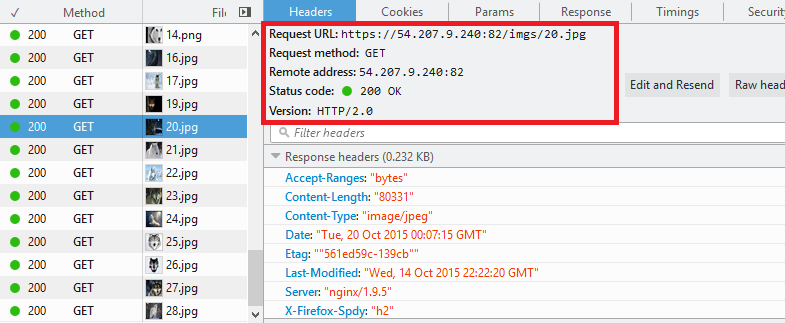
\includegraphics[width=0.7\textwidth]{./04-figuras/desenvolvimento/http2_firefox}
    \label{fig:httpcontenttype2011}
\end{figure}

Esse processo garantiu que o servidor e os navegadores funcionam, pois ambos podem se comunicar utilizando o protocolo HTTP/2. Sendo assim, pôde se dar inicio o processo de realização dos testes.

Como o servidor \textit{nghttpd} não possui um arquivo de configuração, foi necessário colocar cada caso de teste em pastas diferentes e quando um caso novo ia ser testado o servidor tinha de ser reiniciado e apontado para outra pasta.

Para cada técnica de otimização escolhida a página foi carregado 20 vezes utilizando o protocolo HTTP/1.1 no servidor \textit{Nginx} e 20 vezes utilizando o protocolo HTTP/2 no servidor \textit{nghttpd}. Os tempos de carregamentos das páginas foram registrado e foram calculadas as médias e medianas para cada técnica de otimização.